\usetikzlibrary{arrows.meta}
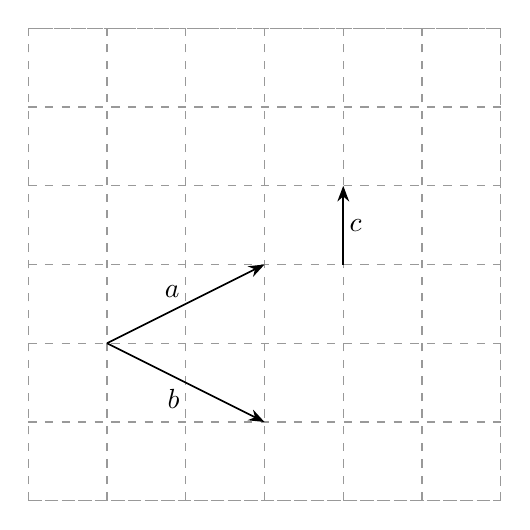
\begin{tikzpicture}[x=10mm,y=10mm,line width=.6pt,font=\normalsize,>=Stealth]
\tikzset{vec/.style={draw=black,line width=.6pt,->,>=Stealth}}
\draw[draw=gray!80,line width=.45pt,dashed] (0,0) grid[xstep=1,ystep=1] (6,6);
\draw[draw=gray!80,line width=.45pt,dashed] (0,0) rectangle (6,6);
\draw[vec] (1,2) -- (3,3);
\draw[vec] (1,2) -- (3,1);
\draw[vec] (4,3) -- (4,4);
\node[inner sep=0pt,anchor=south east,xshift=-2pt,yshift=2pt] at (2,2.5) {$\symbfit{a}$};
\node[inner sep=0pt,anchor=north east,xshift=-2pt,yshift=-2pt] at (2,1.5) {$\symbfit{b}$};
\node[inner sep=0pt,anchor=west,xshift=2pt] at (4,3.5) {$\symbfit{c}$};
\end{tikzpicture}
